\documentclass{article}
\usepackage[a4paper, paperwidth=25cm, paperheight=25.5cm, left=1.5cm, right=1.5cm, top=1cm, bottom=2cm]{geometry}
\usepackage{tikz,tcolorbox}
\usepackage{amsmath}
\usepackage[table,xcdraw]{xcolor}
\usepackage{listings}
\usepackage{array,multirow} % For customizing tables
\usepackage{booktabs} % For better horizontal lines
\usepackage{makecell}
\setlength{\parindent}{0pt}

\lstset{
    language=SQL,                    % Set language to SQL
    basicstyle=\ttfamily\small,      % Font size and family for code
    keywordstyle=\color{blue}\bfseries, % Color for SQL keywords
    commentstyle=\color{gray},       % Color for comments
    stringstyle=\color{red},         % Color for strings
    numbers=left,                    % Show line numbers on the left
    numberstyle=\tiny\color{gray},   % Line number font and color
    stepnumber=1,                    % Line number step
    breaklines=true,                 % Wrap long lines
    frame=single,                    % Add a frame around code
    tabsize=2,                       % Set tab size
    showstringspaces=false           % Hide spaces in strings
}


\newcommand{\ques}[1]{
  \section*{Question #1}
  \vspace{-0.5cm}
  \noindent\rule{\textwidth}{0.5pt}%
}

\newcommand{\tit}[1]{
\begin{center}
    \Large{\textbf{{#1}}}
\end{center}
}

\definecolor{commentgray}{HTML}{676160}
\definecolor{messagegreen}{HTML}{17B867}
\definecolor{myblue}{HTML}{10C2C4}

\tcbuselibrary{skins, breakable, theorems}


\newtcolorbox{prettyBox}[2]{
  enhanced,
  colback=white!90!#2,   % Background color based on the second parameter (color)
  colframe=#2!60!black,  % Frame color based on the second parameter (color)
  coltitle=white,        % Title color (white)
  fonttitle=\bfseries\Large,
  title=#1,              % Title from the first parameter
  boxrule=1mm,
  arc=0.5mm,
  drop shadow=#2!35!gray, % Drop shadow color based on the second parameter (color)
}



\begin{document}
\tit{TP N\(^{\boldsymbol{\circ}}\)\hspace{0.1cm}1}
\ques{1}

\textbf{\underline{Code}}
\lstinputlisting{Questions/q1/q1.sql}

\vspace{1cm}
\textbf{\underline{Output}}
\vspace{1cm}
\begin{center}
    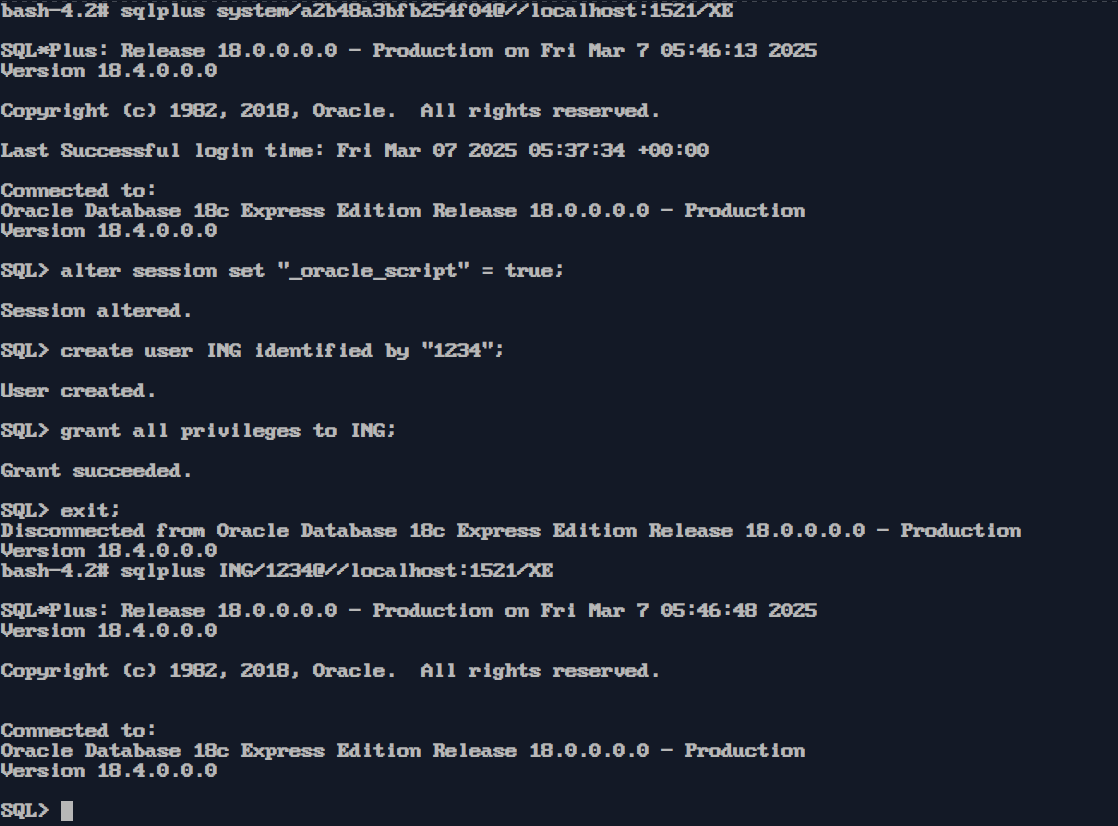
\includegraphics[height=0.5\textheight]{Questions/q1/q1.png}
\end{center}




\newpage
\ques{2}
\textbf{\underline{Code}}
\lstinputlisting{Questions/q2/q2.sql}

\vspace{1cm}
\textbf{\underline{Output}}
\vspace{1cm}
\begin{center}
    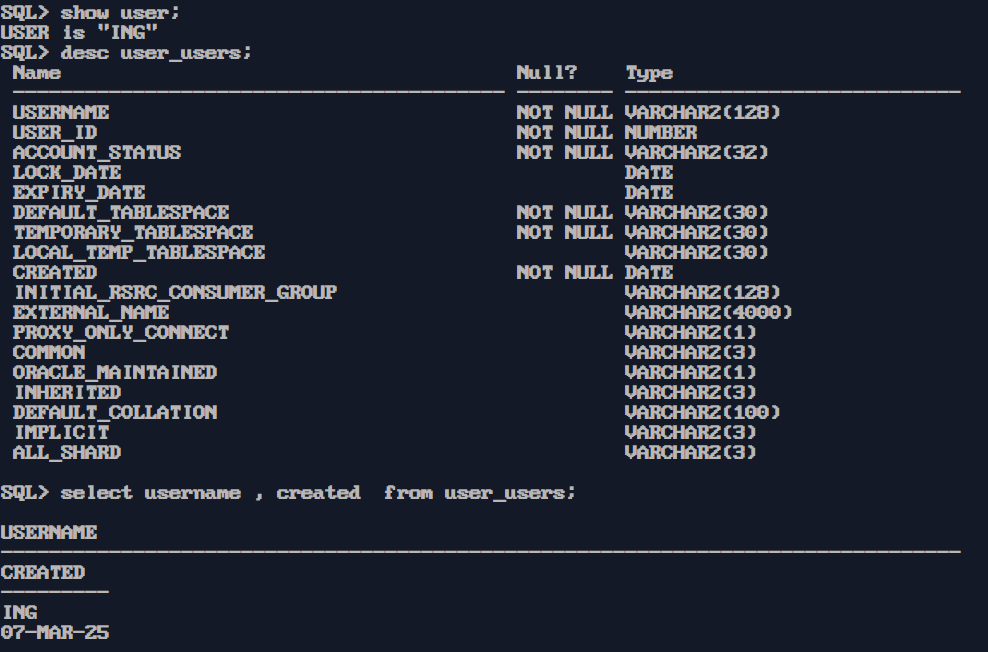
\includegraphics[height=0.5\textheight]{Questions/q2/q2.png}
\end{center}




\newpage
\ques{3}
\textbf{\underline{Code}}\\[0.1cm]
\textbf{\underline{Usine}}
\lstinputlisting[firstline=1,lastline=7]{Questions/q3/q3.sql}

\vspace{0.25cm}
\textbf{\underline{Produit}}
\lstinputlisting[firstline=9,lastline=17]{Questions/q3/q3.sql}

\vspace{0.25cm}
\textbf{\underline{Fournisseur}}
\lstinputlisting[firstline=19,lastline=29]{Questions/q3/q3.sql}

\vspace{0.25cm}
\textbf{\underline{Livraison}}
\lstinputlisting[firstline=31]{Questions/q3/q3.sql}




\newpage
\ques{4}
\textbf{\underline{Code}}
\lstinputlisting{Questions/q4/q4.sql}

\vspace{1cm}
\textbf{\underline{Output}}
\vspace{1cm}
\begin{center}
    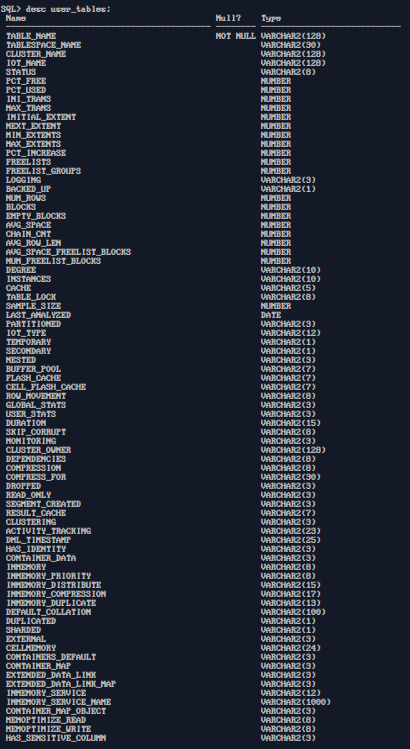
\includegraphics[height=0.5\textheight]{Questions/q4/desc.png}
    
    \vspace{0.25cm}
    
    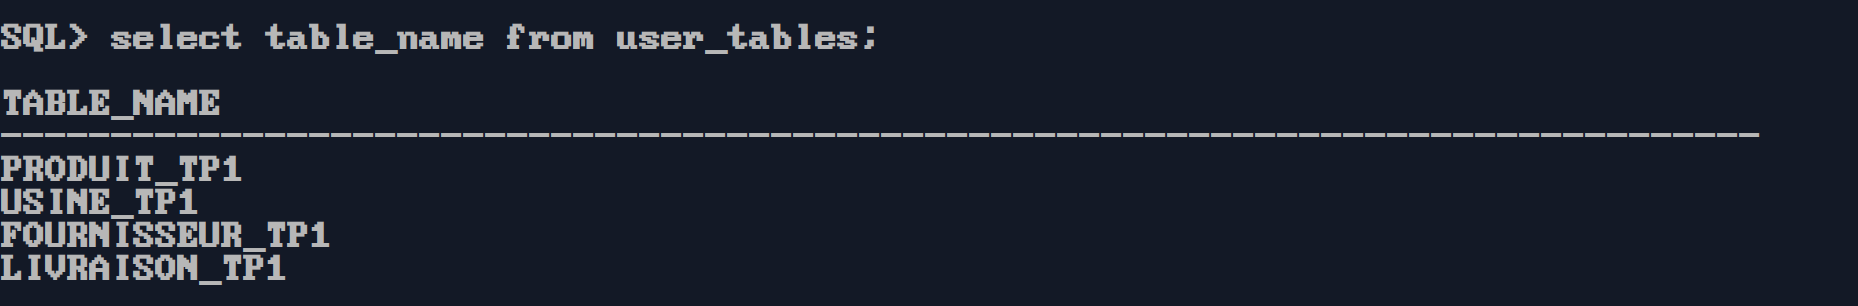
\includegraphics[height=0.15\textheight]{Questions/q4/name.png}
\end{center}






\newpage
\ques{5}
\textbf{\underline{Code}}
\lstinputlisting{Questions/q5/q5.sql}

\vspace{1cm}
\textbf{\underline{Output}}
\vspace{1cm}
\begin{center}
    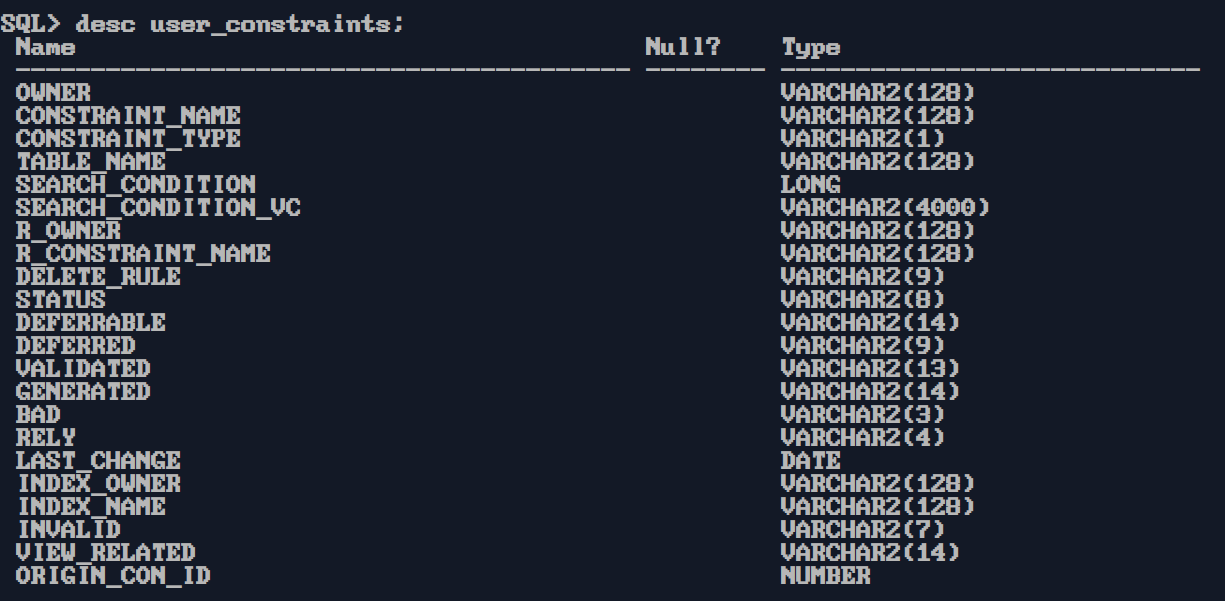
\includegraphics[height=0.3\textheight]{Questions/q5/desc.png}
    
    \vspace{0.25cm}
    
    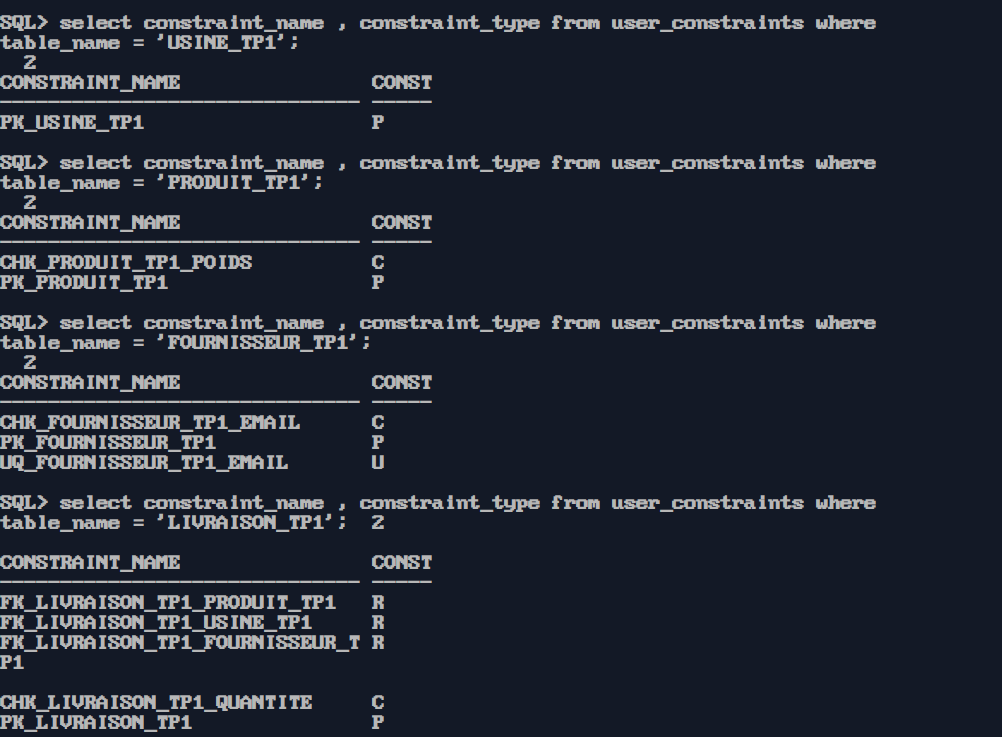
\includegraphics[height=0.4\textheight]{Questions/q5/const.png}
\end{center}



\newpage
\ques{6}
\textbf{\underline{Code}}
\lstinputlisting{Questions/q6/q6.sql}

\vspace{1cm}
\textbf{\underline{Output}}
\vspace{1cm}
\begin{center}
    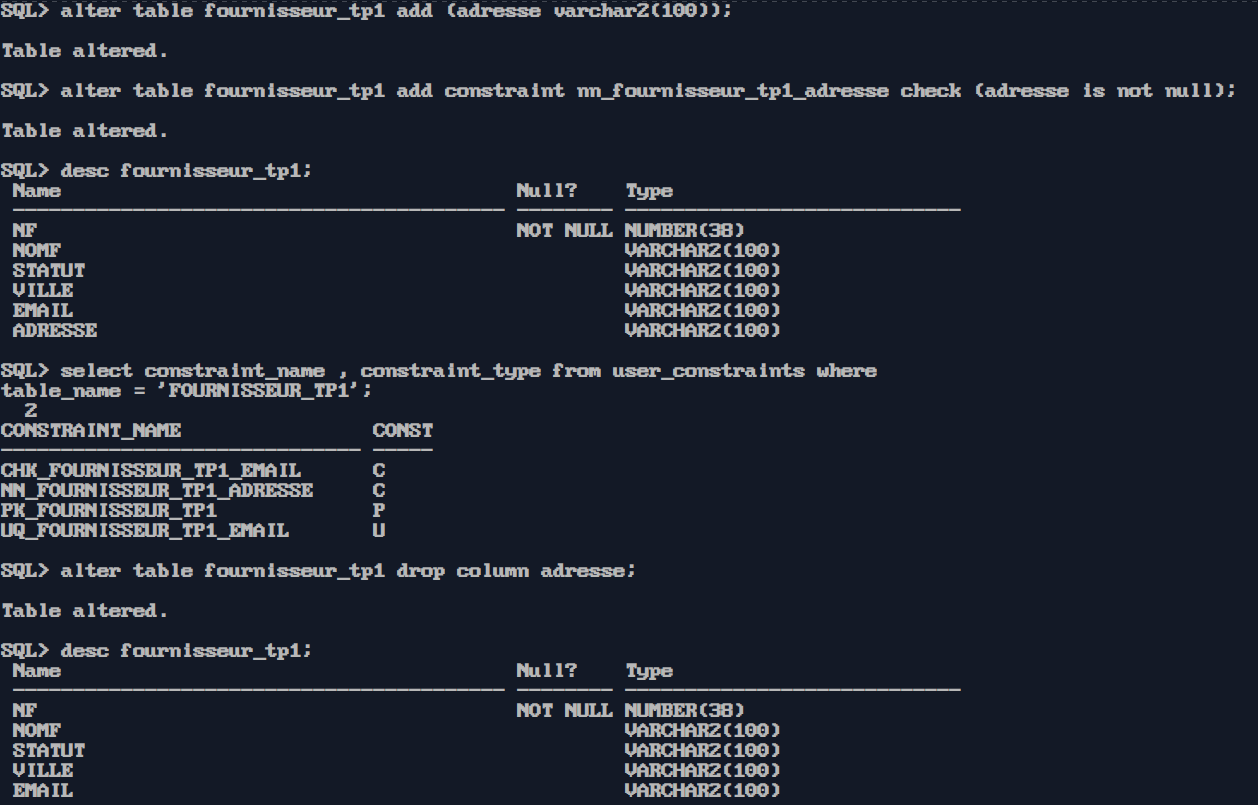
\includegraphics[height=0.4\textheight]{Questions/q6/ad.png}
\end{center}



\newpage
\ques{7}
\textbf{\underline{Code}}
\lstinputlisting{Questions/q7/q7.sql}



\newpage
\ques{8}

\textbf{\underline{Code}}
\lstinputlisting{Questions/q8/q8.sql}

\vspace{1cm}
\textbf{\underline{Output}}
\vspace{1cm}
\begin{center}
    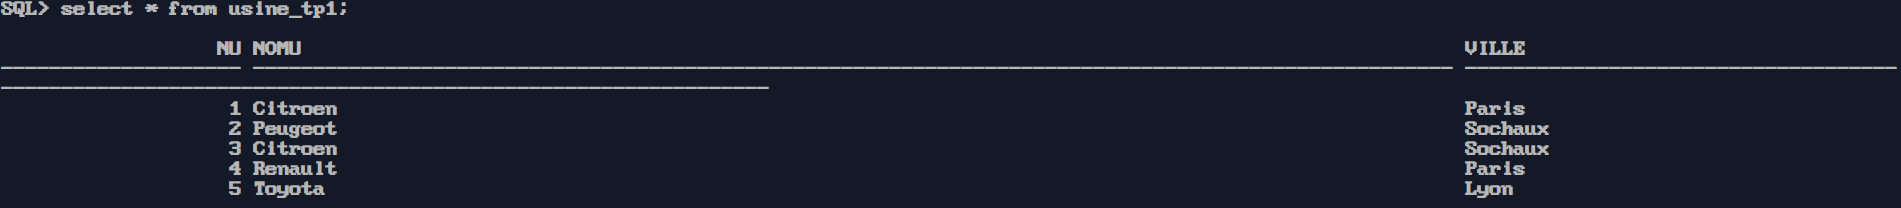
\includegraphics[width=0.9\textwidth]{Questions/q8/q8.png}
\end{center}




\newpage
\ques{9}

\textbf{\underline{Code}}
\lstinputlisting{Questions/q9/q9.sql}

\vspace{1cm}
\textbf{\underline{Output}}
\vspace{1cm}
\begin{center}
    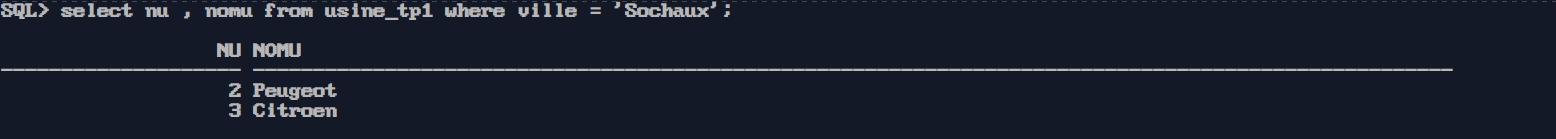
\includegraphics[width=0.9\textwidth]{Questions/q9/q9.png}
\end{center}



\newpage
\ques{10}

\textbf{\underline{Code}}
\lstinputlisting{Questions/q10/q10.sql}

\vspace{1cm}
\textbf{\underline{Output}}
\vspace{1cm}
\begin{center}
    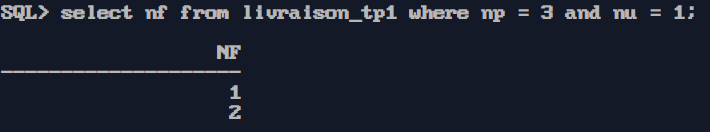
\includegraphics[width=0.9\textwidth]{Questions/q10/q10.png}
\end{center}



\newpage
\ques{11}

\textbf{\underline{Code}}
\lstinputlisting{Questions/q11/q11.sql}

\vspace{1cm}
\textbf{\underline{Output}}
\vspace{1cm}
\begin{center}
    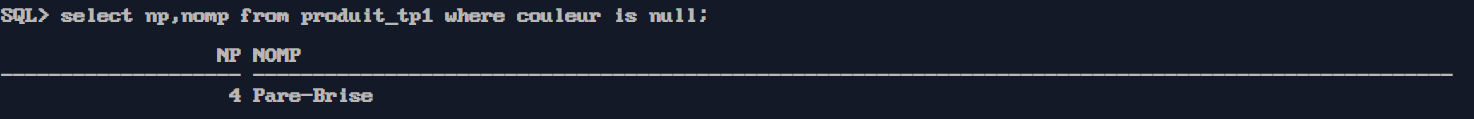
\includegraphics[width=0.9\textwidth]{Questions/q11/q11.png}
\end{center}



\newpage
\ques{12}

\textbf{\underline{Code}}
\lstinputlisting{Questions/q12/q12.sql}

\vspace{1cm}
\textbf{\underline{Output}}
\vspace{1cm}
\begin{center}
    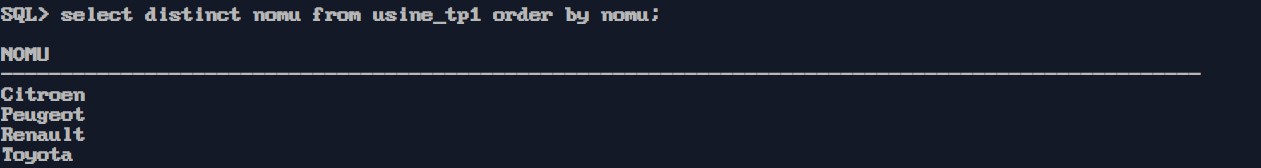
\includegraphics[width=0.9\textwidth]{Questions/q12/q12.png}
\end{center}



\newpage
\ques{13}

\textbf{\underline{Code}}
\lstinputlisting{Questions/q13/q13.sql}

\vspace{1cm}
\textbf{\underline{Output}}
\vspace{1cm}
\begin{center}
    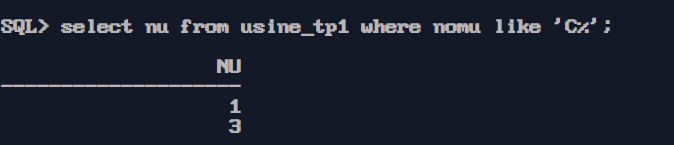
\includegraphics[width=0.9\textwidth]{Questions/q13/q13.png}
\end{center}



\newpage
\ques{14}

\textbf{\underline{Code}}
\lstinputlisting{Questions/q14/q14.sql}

\vspace{1cm}
\textbf{\underline{Output}}
\vspace{1cm}
\begin{center}
    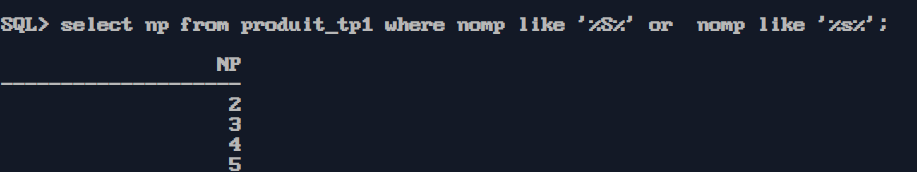
\includegraphics[width=0.9\textwidth]{Questions/q14/q14.png}
\end{center}



\newpage
\ques{15}

\textbf{\underline{Code}}
\lstinputlisting{Questions/q15/q15.sql}

\vspace{1cm}
\textbf{\underline{Output}}
\vspace{1cm}
\begin{center}
    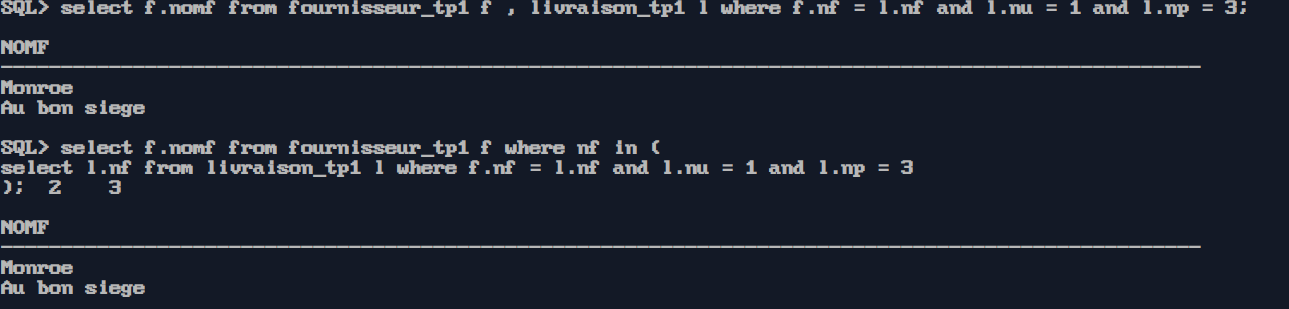
\includegraphics[width=0.9\textwidth]{Questions/q15/q15.png}
\end{center}



\newpage
\ques{16}

\textbf{\underline{Code}}
\lstinputlisting{Questions/q16/q16.sql}

\vspace{1cm}
\textbf{\underline{Output}}
\vspace{1cm}
\begin{center}
    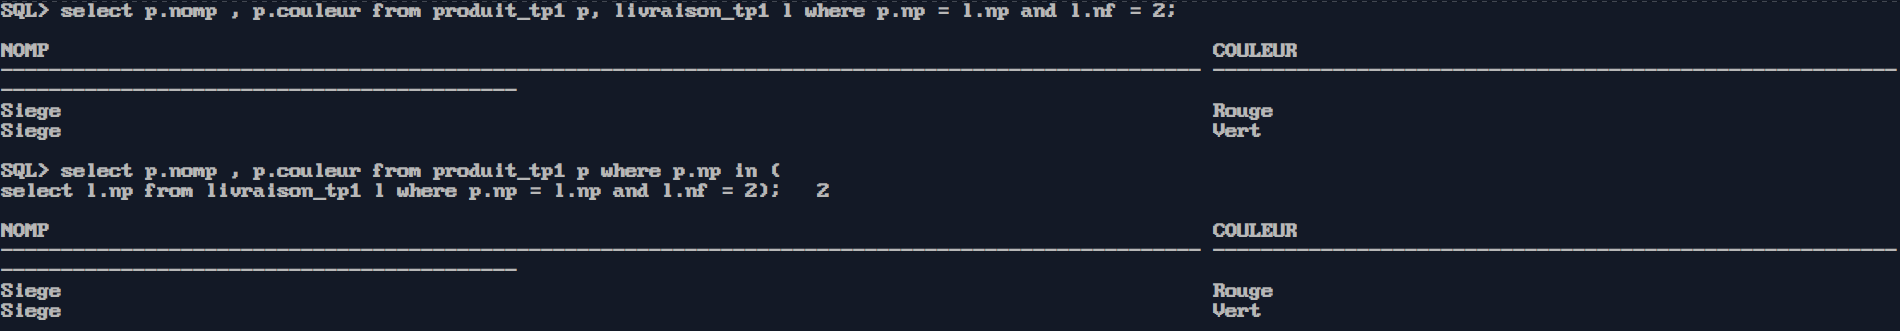
\includegraphics[width=0.9\textwidth]{Questions/q16/q16.png}
\end{center}



\newpage
\ques{17}

\textbf{\underline{Code}}
\lstinputlisting{Questions/q17/q17.sql}

\vspace{1cm}
\textbf{\underline{Output}}
\vspace{1cm}
\begin{center}
    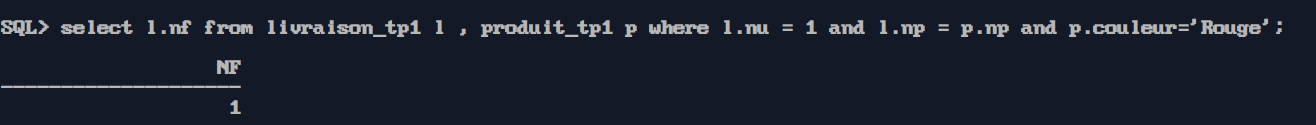
\includegraphics[width=0.9\textwidth]{Questions/q17/q17.png}
\end{center}



\newpage
\ques{18}

\textbf{\underline{Code}}
\lstinputlisting{Questions/q18/q18.sql}

\vspace{1cm}
\textbf{\underline{Output}}
\vspace{1cm}
\begin{center}
    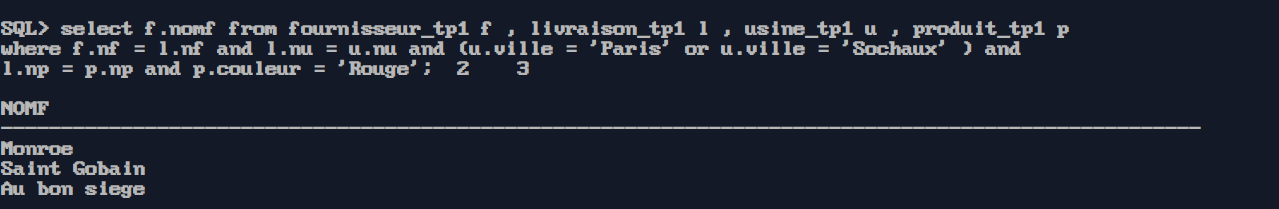
\includegraphics[width=0.9\textwidth]{Questions/q18/q18.png}
\end{center}



\newpage
\ques{19}

\textbf{\underline{Code}}
\lstinputlisting{Questions/q19/q19.sql}

\vspace{1cm}
\textbf{\underline{Output}}
\vspace{1cm}
\begin{center}
    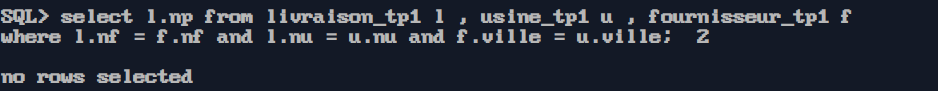
\includegraphics[width=0.9\textwidth]{Questions/q19/q19.png}
\end{center}



\newpage
\ques{20}

\textbf{\underline{Code}}
\lstinputlisting{Questions/q20/q20.sql}

\vspace{1cm}
\textbf{\underline{Output}}
\vspace{1cm}
\begin{center}
    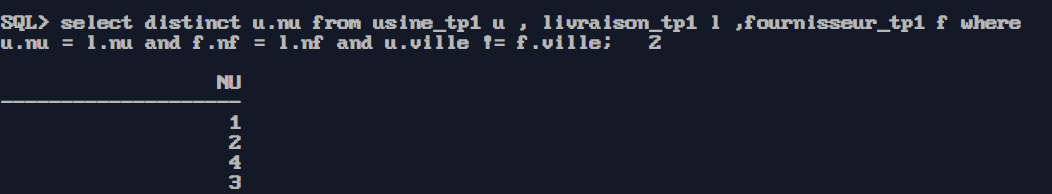
\includegraphics[width=0.9\textwidth]{Questions/q20/q20.png}
\end{center}



\newpage
\ques{21}

\textbf{\underline{Code}}
\lstinputlisting{Questions/q21/q21.sql}

\vspace{1cm}
\textbf{\underline{Output}}
\vspace{1cm}
\begin{center}
    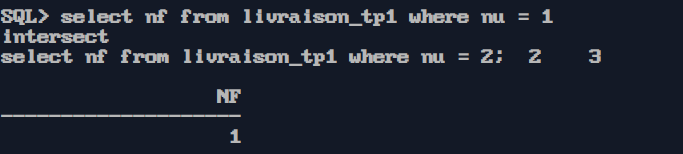
\includegraphics[width=0.9\textwidth]{Questions/q21/q21.png}
\end{center}



\newpage
\ques{22}

\textbf{\underline{Code}}
\lstinputlisting{Questions/q22/q22.sql}

\vspace{1cm}
\textbf{\underline{Output}}
\vspace{1cm}
\begin{center}
    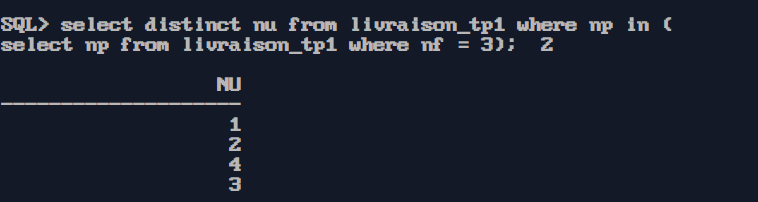
\includegraphics[width=0.9\textwidth]{Questions/q22/q22.png}
\end{center}



\newpage
\ques{23}

\textbf{\underline{Code}}
\lstinputlisting{Questions/q23/q23.sql}

\vspace{1cm}
\textbf{\underline{Output}}
\vspace{1cm}
\begin{center}
    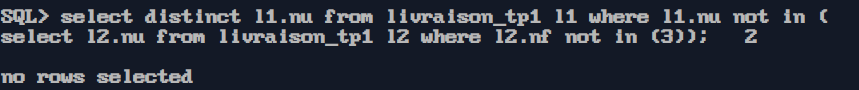
\includegraphics[width=0.9\textwidth]{Questions/q23/q23.png}
\end{center}



\newpage
\ques{24}

\textbf{\underline{Code}}
\lstinputlisting{Questions/q24/q24.sql}

\vspace{1cm}
\textbf{\underline{Output}}
\vspace{1cm}
\begin{center}
    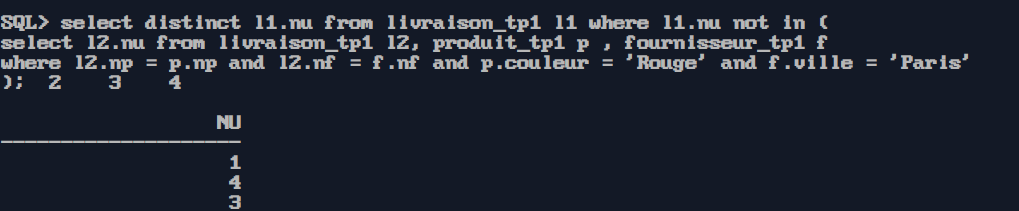
\includegraphics[width=0.9\textwidth]{Questions/q24/q24.png}
\end{center}



\newpage
\ques{25}

\textbf{\underline{Code}}
\lstinputlisting{Questions/q25/q25.sql}

\vspace{1cm}
\textbf{\underline{Output}}
\vspace{1cm}
\begin{center}
    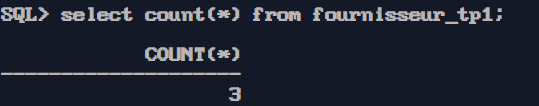
\includegraphics[width=0.9\textwidth]{Questions/q25/q25.png}
\end{center}



\newpage
\ques{26}

\textbf{\underline{Code}}
\lstinputlisting{Questions/q26/q26.sql}

\vspace{1cm}
\textbf{\underline{Output}}
\vspace{1cm}
\begin{center}
    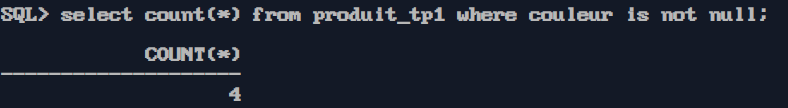
\includegraphics[width=0.9\textwidth]{Questions/q26/q26.png}
\end{center}



\newpage
\ques{27}

\textbf{\underline{Code}}
\lstinputlisting{Questions/q27/q27.sql}

\vspace{1cm}
\textbf{\underline{Output}}
\vspace{1cm}
\begin{center}
    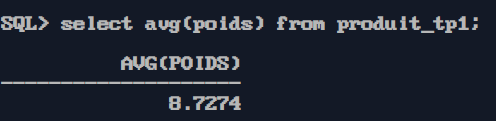
\includegraphics[width=0.9\textwidth]{Questions/q27/q27.png}
\end{center}



\newpage
\ques{28}

\textbf{\underline{Code}}
\lstinputlisting{Questions/q28/q28.sql}

\vspace{1cm}
\textbf{\underline{Output}}
\vspace{1cm}
\begin{center}
    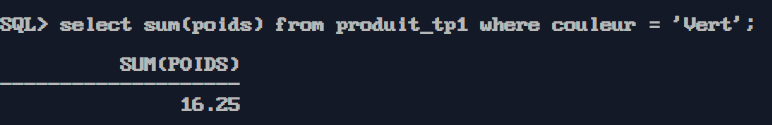
\includegraphics[width=0.9\textwidth]{Questions/q28/q28.png}
\end{center}



\newpage
\ques{29}

\textbf{\underline{Code}}
\lstinputlisting{Questions/q29/q29.sql}

\vspace{1cm}
\textbf{\underline{Output}}
\vspace{1cm}
\begin{center}
    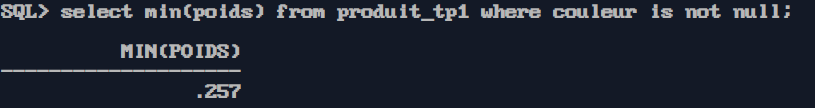
\includegraphics[width=0.9\textwidth]{Questions/q29/q29.png}
\end{center}



\newpage
\ques{30}

\textbf{\underline{Code}}
\lstinputlisting{Questions/q30/q30.sql}

\vspace{1cm}
\textbf{\underline{Output}}
\vspace{1cm}
\begin{center}
    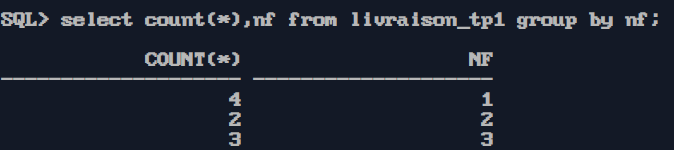
\includegraphics[width=0.9\textwidth]{Questions/q30/q30.png}
\end{center}



\newpage
\ques{31}

\textbf{\underline{Code}}
\lstinputlisting{Questions/q31/q31.sql}

\vspace{1cm}
\textbf{\underline{Output}}
\vspace{1cm}
\begin{center}
    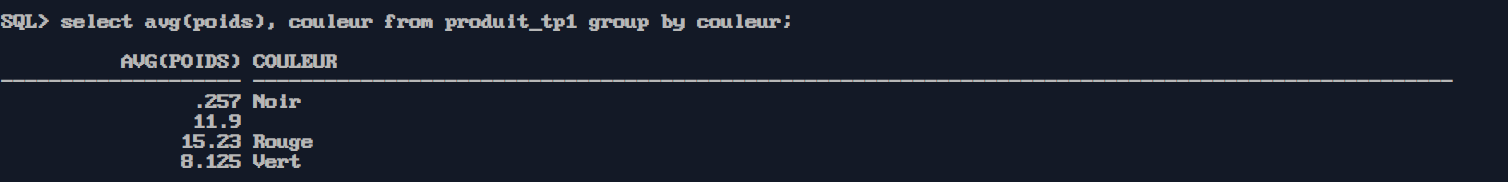
\includegraphics[width=0.9\textwidth]{Questions/q31/q31.png}
\end{center}



\newpage
\ques{32}

\textbf{\underline{Code}}
\lstinputlisting{Questions/q32/q32.sql}

\vspace{1cm}
\textbf{\underline{Output}}
\vspace{1cm}
\begin{center}
    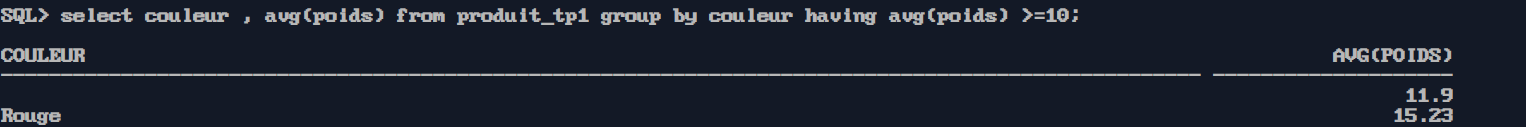
\includegraphics[width=0.9\textwidth]{Questions/q32/q32.png}
\end{center}



\newpage
\ques{33}

\textbf{\underline{Code}}
\lstinputlisting{Questions/q33/q33.sql}

\vspace{1cm}
\textbf{\underline{Output}}
\vspace{1cm}
\begin{center}
    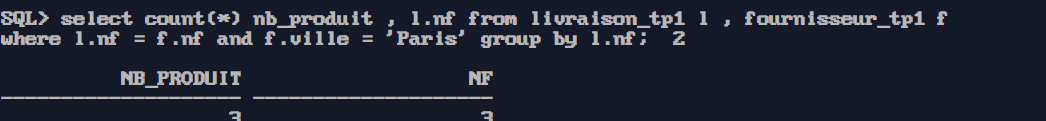
\includegraphics[width=0.9\textwidth]{Questions/q33/q33.png}
\end{center}



\newpage
\ques{34}

\textbf{\underline{Code}}
\lstinputlisting{Questions/q34/q34.sql}

\vspace{1cm}
\textbf{\underline{Output}}
\vspace{1cm}
\begin{center}
    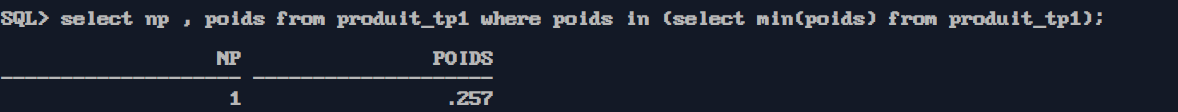
\includegraphics[width=0.9\textwidth]{Questions/q34/q34.png}
\end{center}



\newpage
\ques{35}

\textbf{\underline{Code}}
\lstinputlisting{Questions/q35/q35.sql}

\vspace{1cm}
\textbf{\underline{Output}}
\vspace{1cm}
\begin{center}
    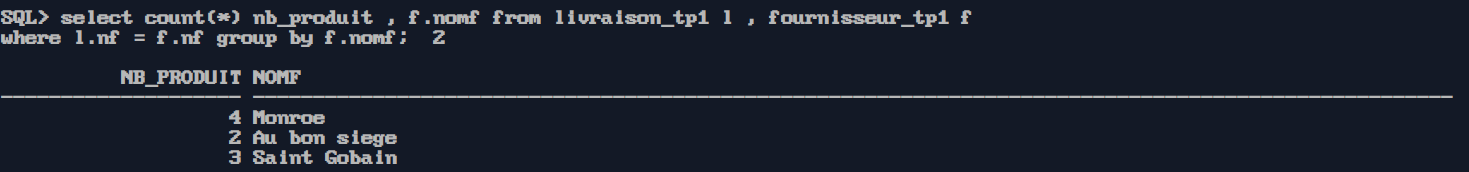
\includegraphics[width=0.9\textwidth]{Questions/q35/q35.png}
\end{center}



\newpage
\ques{36}

\textbf{\underline{Code}}
\lstinputlisting{Questions/q36/q36.sql}

\vspace{1cm}
\textbf{\underline{Output}}
\vspace{1cm}
\begin{center}
    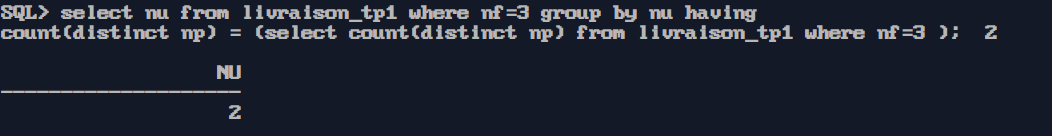
\includegraphics[width=0.9\textwidth]{Questions/q36/q36.png}
\end{center}



\newpage
\ques{37}

\textbf{\underline{Code}}
\lstinputlisting{Questions/q37/q37.sql}

\vspace{1cm}
\textbf{\underline{Output}}
\vspace{1cm}
\begin{center}
    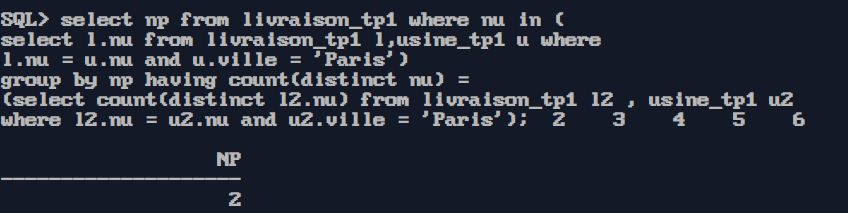
\includegraphics[width=0.9\textwidth]{Questions/q37/q37.png}
\end{center}



\newpage
\ques{38}

\textbf{\underline{Code}}
\lstinputlisting{Questions/q38/q38.sql}

\vspace{1cm}
\textbf{\underline{Output}}
\vspace{1cm}
\begin{center}
    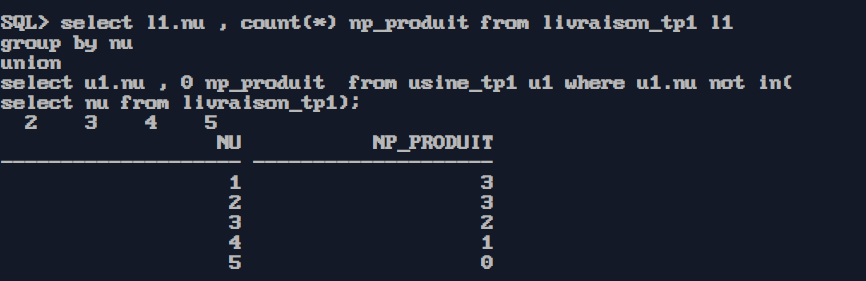
\includegraphics[width=0.9\textwidth]{Questions/q38/q38.png}
\end{center}



\newpage
\ques{39}

\textbf{\underline{Code}}
\lstinputlisting{Questions/q39/q39.sql}

\vspace{1cm}
\textbf{\underline{Output}}
\vspace{1cm}
\begin{center}
    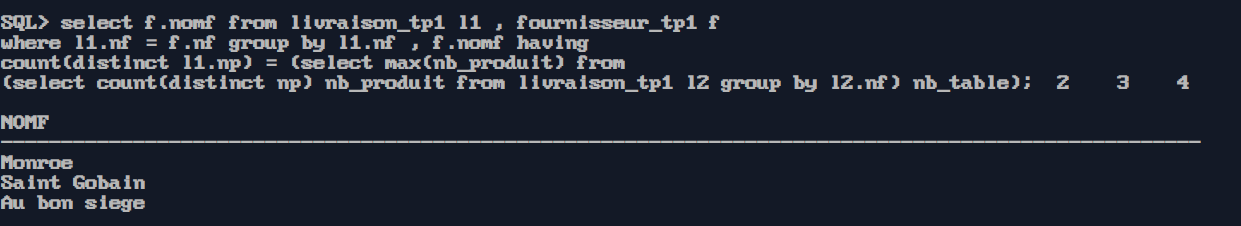
\includegraphics[width=0.9\textwidth]{Questions/q39/q39.png}
\end{center}



\newpage
\ques{40}

\textbf{\underline{Code}}
\lstinputlisting{Questions/q40/q40.sql}

\vspace{1cm}
\textbf{\underline{Output}}
\vspace{1cm}
\begin{center}
    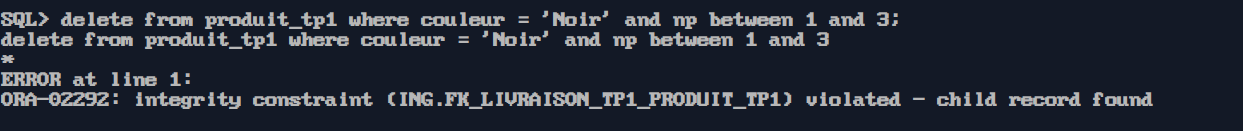
\includegraphics[width=0.9\textwidth]{Questions/q40/q40.png}
\end{center}



\newpage
\ques{41}

\textbf{\underline{Code}}
\lstinputlisting{Questions/q41/q41.sql}

\vspace{1cm}
\textbf{\underline{Output}}
\vspace{1cm}
\begin{center}
    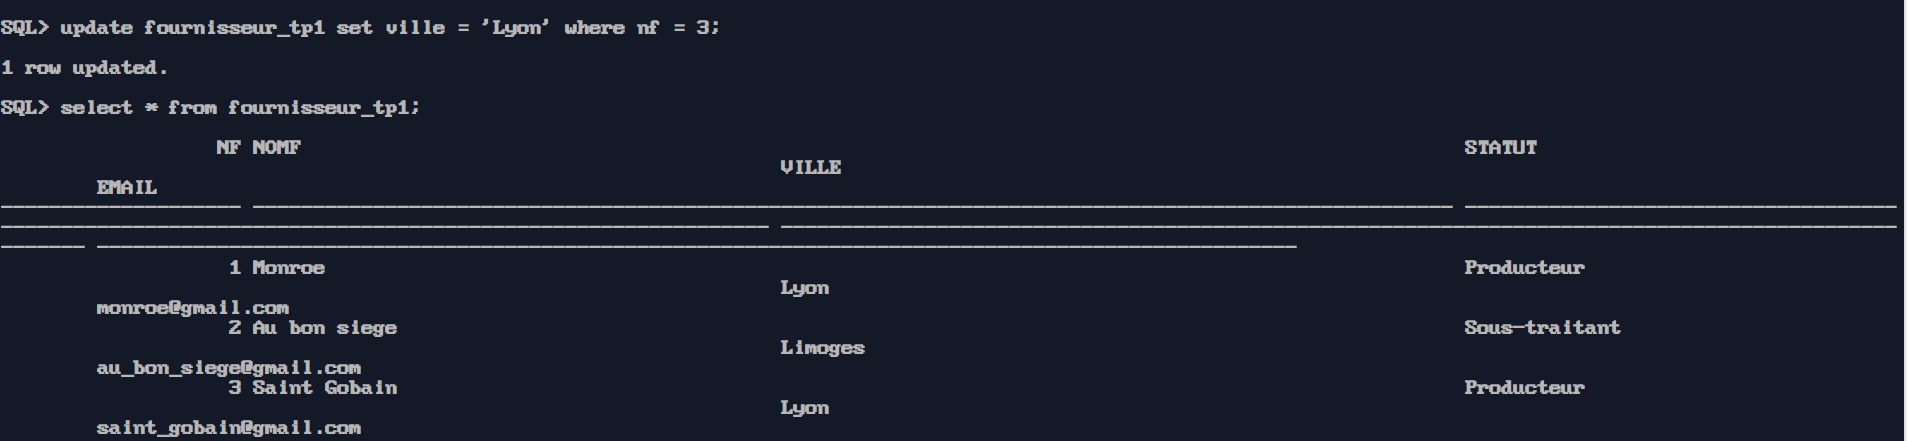
\includegraphics[width=0.9\textwidth]{Questions/q41/q41.png}
\end{center}

\newpage
\ques{42}

\textbf{\underline{Code}}
\lstinputlisting{Questions/q42/q42.sql}

\vspace{1cm}
\textbf{\underline{Output}}
\vspace{1cm}
\begin{center}
    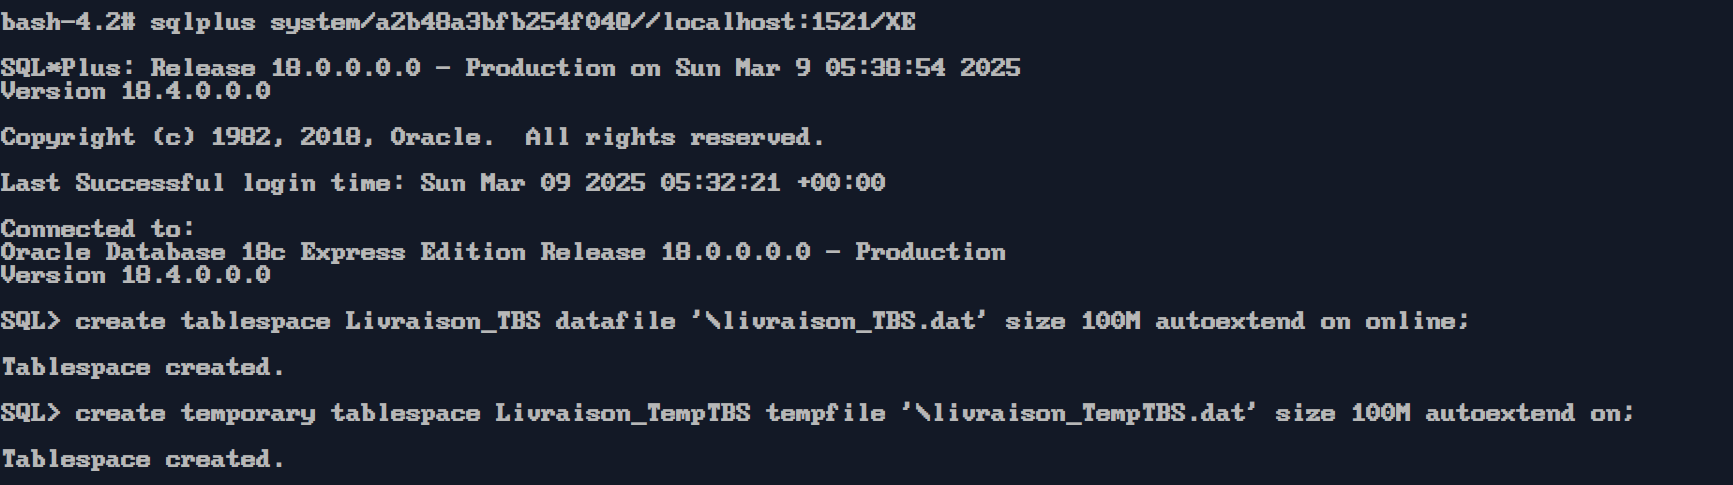
\includegraphics[width=0.9\textwidth]{Questions/q42/q42.png}
\end{center}


\newpage
\ques{43}

\textbf{\underline{Code}}
\lstinputlisting{Questions/q43/q43.sql}

\vspace{1cm}
\textbf{\underline{Output}}
\vspace{1cm}
\begin{center}
    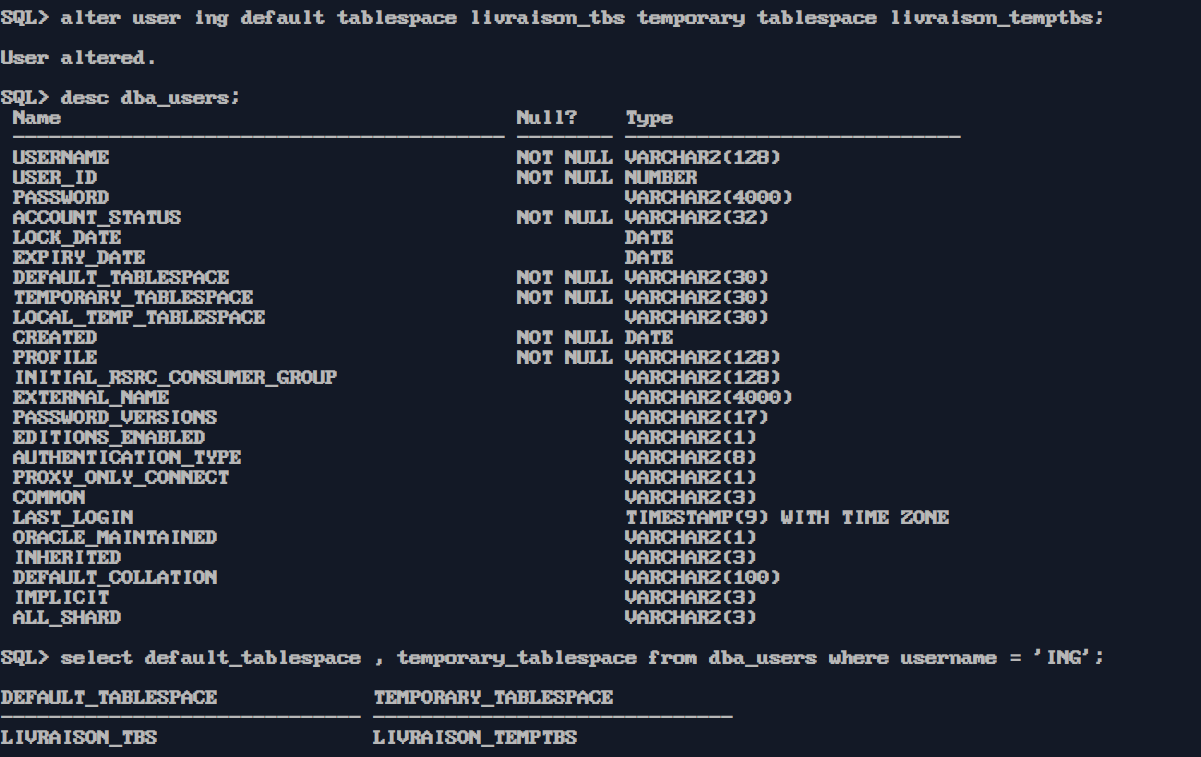
\includegraphics[width=0.9\textwidth]{Questions/q43/q43.png}
\end{center}


\newpage
\ques{44}

\textbf{\underline{Code}}
\lstinputlisting{Questions/q44/q44.sql}



\newpage
\ques{45}

\textbf{\underline{Code}}
\lstinputlisting{Questions/q45/q45.sql}



\newpage
\ques{46}

\textbf{\underline{Code}}
\lstinputlisting{Questions/q46/q46.sql}

\vspace{1cm}
\textbf{\underline{Output}}
\vspace{1cm}
\begin{center}
    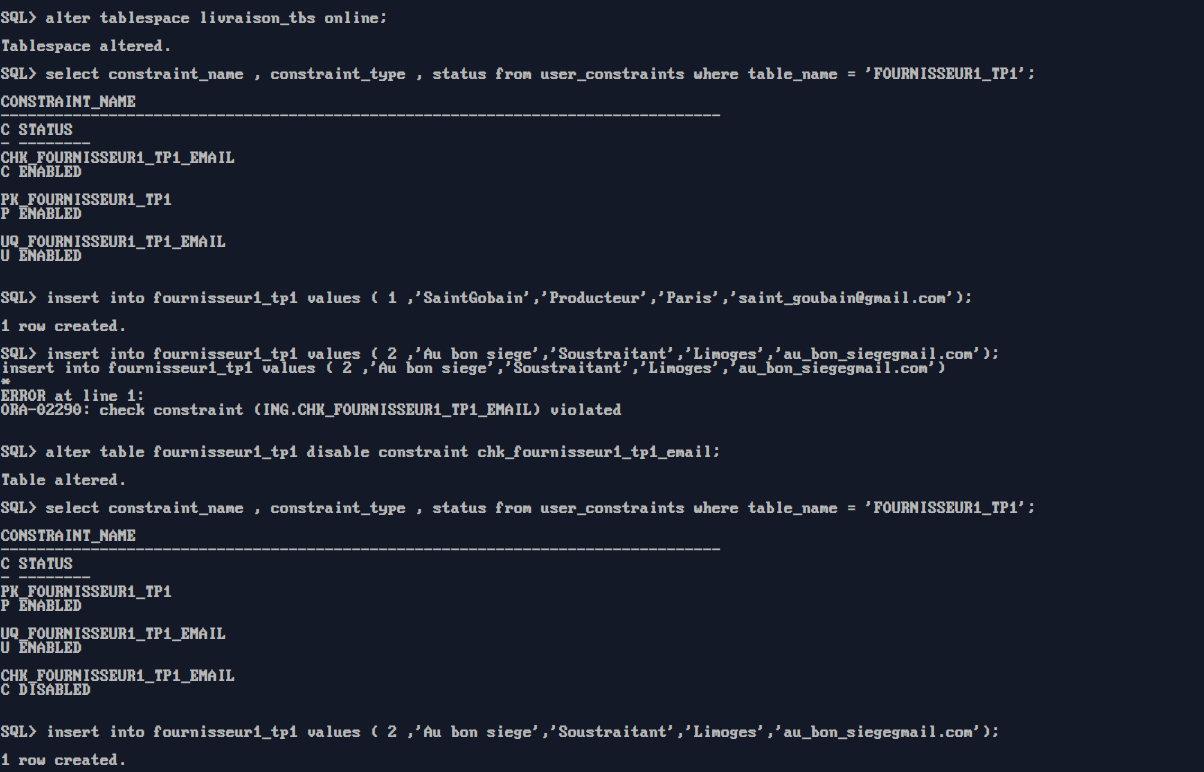
\includegraphics[width=0.8\textwidth]{Questions/q46/q46.png}
\end{center}


\newpage
\ques{47}

\textbf{\underline{Code}}
\lstinputlisting{Questions/q47/q47.sql}

\newpage
\textbf{\underline{Output}}
\vspace{1cm}
\begin{center}
    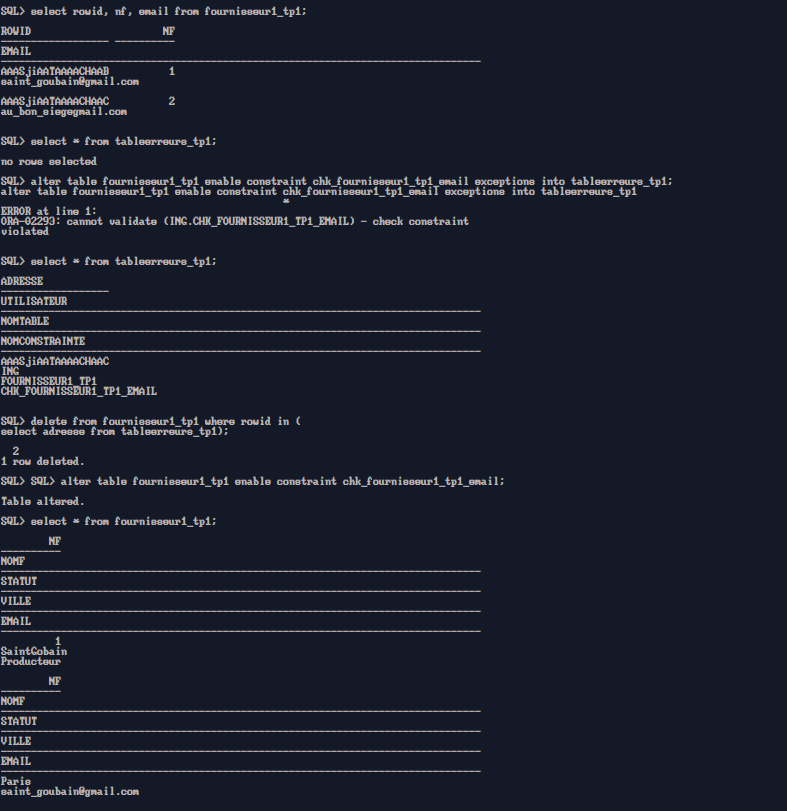
\includegraphics[width=0.8\textwidth]{Questions/q47/q47.png}
\end{center}


\end{document}
